\lecture{9}{Триангуляция Делоне. ЕМОД.}
\subsection{Триангуляция Делоне.}
\begin{definition}
  \highlight{Триангуляция} --- планарный граф, все внутренние области которого являются треугольниками. 
\end{definition}

\begin{definition}
  \highlight{Выпуклая триангуляция} --- триангуляция, для которой минимальный многоугольник, охватывающий
  все треугольники, будет выпуклым.
\end{definition}

\begin{definition}
  Триангуляция удовлетворяет \highlight{условию Делоне}, если внутри окружности, описанной вокруг
  любого построенного треугольника, не попадает ни одна из заданных точек триангуляции.
\end{definition}

\begin{definition}
  \highlight{Триангуляция Делоне} --- выпуклая триангуляция, которая удовлетворяет условию Делоне.
\end{definition}

\begin{figure}[H]    
  \centering    
  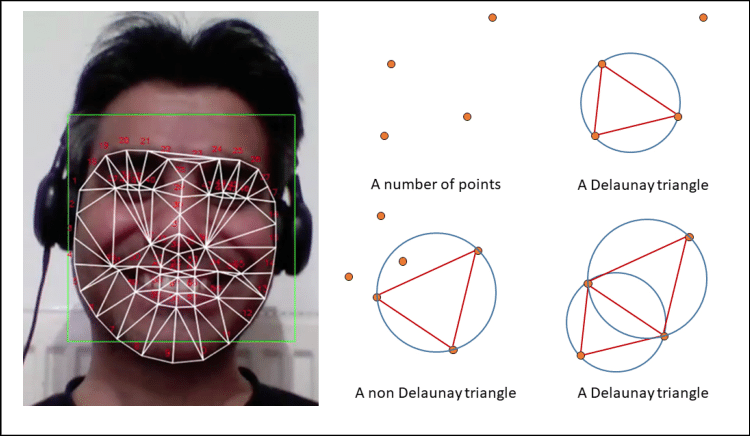
\includegraphics[width=0.8\textwidth]{figures/deloneExample.png}    
  \caption*{Пример триангуляций}        
\end{figure} 

Существует множество алгоритмов построения триангуляции Делоне за $O(n \log n)$ и $O(n^2)$. 
Приведем пример алгоритма <<Удаляй и строй>>.
Построение происходит итеративно, опишем процесс вставки очередной вершины:
\begin{enumerate}
  \item Находим треугольники, в описанные окружности которых входит новая точка (это можно делать, например,
    задачей локализации точки, а потом проверкой смежных треугольников)
  \item Удаляем эти треугольники, образуется многоугольник с точкой внутри (случай б на рисунке)
  \item Соединяем новую точку с вершинами образованного многоугольника
\end{enumerate}

\begin{figure}[H]    
  \centering    
  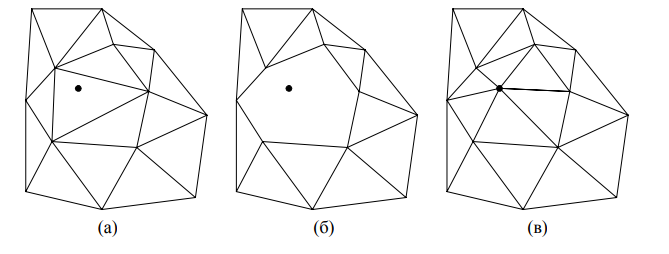
\includegraphics[width=0.8\textwidth]{figures/deloneConstruct.png}    
  \caption*{<<Удаляй и строй>>}        
\end{figure} 

\begin{remark}
  Асимптотика такого алгоритма $O(n^2)$.
\end{remark}
\begin{proof}
  Первый пункт алгоритма (поиск треугольника) можно делать обходом всех треугольников за $O(n)$, нахождение
  треугольников для удаление также за $O(n)$, итого получаем  $O(n^2)$.
\end{proof}

\subsection{Связь триангуляции с выпуклой оболочкой.}
Спроектируем точки плоскости на параболоид так, что
\[
  (x, y) \to (X, Y, Z), X = x, Y = y, Z = x^2 + y^2
.\] 

Заметим, что в таком случае проекция триангуляции Делоне на параболоид является её нижняя выпуклая оболочка.
Проведём плоскость через три точки триангуляции Делоне на параболоиде. Плоскость сечёт параболоид
по эллипсу, который в проекции на плоскость даст окружность. По свойству триангуляции Делоне внутри
этой окружности нет других точек множества. Следовательно на параболоиде все точки множества лежат
по одну сторону от плоскости трёх спроектированных точек. Поясним последний переход подробнее.

Пусть рассматриваемая окружность имеет уравнение:
\[
  x^2 + y^2 + ax + by + c = 0
.\] 
При переходе к параболоиду с заменой $X = x, Y = y, Z = x^2 + y^2$ получаем:
\[
  aX + bY + Z + c = 0
.\] 
Что соответствует уравнению плоскости, которое как раз определяет относительное положение других точек и
плоскости.
\begin{figure}[H]    
  \centering    
  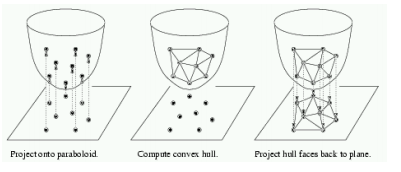
\includegraphics[width=0.8\textwidth]{figures/deloneConvex.png}    
  \caption*{Связь триангуляции Делоне и выпуклой оболочки}        
\end{figure} 

\subsection{ЕМОД.}
Пусть на плоскости задано множество из $n$ точек.
\begin{definition}
  \highlight{Евклидово минимальное остовное дерево (ЕМОД)} --- минимальное остовное дерево в полном
  взвешенном графе на данном множестве точек, где вес ребра --- евклидово расстояние между точками.
\end{definition}

Наивное построение с помощью обычных алгоритмов построения MST (Прим, Крускал, Борувка) за $O(n^2 \log n)$,
т.к. граф полный ($E = O(n^2)$).

Построим ЕМОД с помощью триангуляции Делоне:
\begin{enumerate}
  \item Строим триангуляцию Делоне за $O(n \log n)$
  \item Находим MST на построенной триангуляции обычным алгоритмом (Прим, Крускал, Борувка) за 
    $O(n \log n)$ --- получаем ЕМОД за чудесные $O(n \log n)$.
\end{enumerate}

\begin{figure}[H]    
  \centering    
  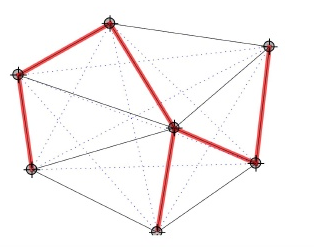
\includegraphics[width=0.5\textwidth]{figures/deloneMST.png}    
  \caption*{Пример нахождения ЕМОД с помощью триангуляции}        
\end{figure} 

Осталось доказать, что любое ЕМОД содержит только рёбра триангуляции и никакие другие.
(очень мутная теорема)
\begin{theorem}
  Любое ребро, не входящее в триангуляцию Делоне, не содержится ни в каком EMST.  
\end{theorem}
\begin{proof}
  Рассмотрим ребро $e$ между точками $p$ и $q$, которое не является ребром триангуляции Делоне.
  Верно следующее утверждение: если существует цикл с двумя входными точками на границе, 
  который не содержит других входных точек, отрезок между этими точками является ребром любой триангуляции
  Делоне. Из этого утверждения вытекает, что цикл $C$ с $e$ в качестве диаметра должен содержать
  некоторую другую точку $r$ внутри. Но тогда $r$ ближе к $p$ и $q$, чем они по отношению друг к другу.
  Значит $pq$ является самым длинным ребром в цикле $p \to  q \to r \to p$, а значит, что не принадлежит
  никакому $EMST$.
\end{proof}




